\section{Regenradar Vorhersage}
Ziel dieser Aufgabe ist es, mit Hilfe eines UNets eine kurzzeit-Regenvorhersage zu erreichen. Die hier verwendeten Daten sind im Kapitel \ref{Samples} genauer erklärt. Ziel des Netzes ist es die Baseline zu schlagen. Als Baseline zählen wir die Vorhersage des zeitlich Letzten Bildes. Es wird bei der Baseline also davon ausgegangen, dass sich an dem Regenverhalten nichts ändert. Im ersten Unterkapitel wird das UNet verwendet um eine fünf-minuten Vorhersage zu machen. Es werden verschiedene Erweiterungen an dem bisherigen UNet angewandt um eine eventuelle performance Steigerung zu erreichen. Im zweiten Unterkapitel soll eine Vorhersage bis zu 35 Minuten in die ZUkunft möglich werden. Die Auswertung wird im jeweiligen Kapitel vorgenommen.

\subsection{Fünf Minuten vorhersage}
Um eine Radar-Vorhersage für fünf Minuten zu erreichen, werden Daten wie in Kapitel \ref{Samples} in Abbildung \ref{5D1L} gezeigt verwendet. Die Eingabedaten bestehen aus fünf aufeinander folgende Bilder, welche bis zu 20 Minuten in die Vergangenheit reichen. Das Radarbild im Label ist 5 Minuten in der Zukunft.

Die verwendete Architektur entspricht der des in Kapitel \ref{kapitelUNet} beschriebenen UNets. Die verwendete Fehlerfunktion ist der MSE. Das Training beschränkt sich auf 1900 Samples aus dem Jahr 2016, zum validieren wurden die letzten 50 Samples aus dem Dezember genommen. Die Validierungsdaten kommen somit in keiner Weise während des Trainings vor.
\begin{figure}[h]
	\centering
	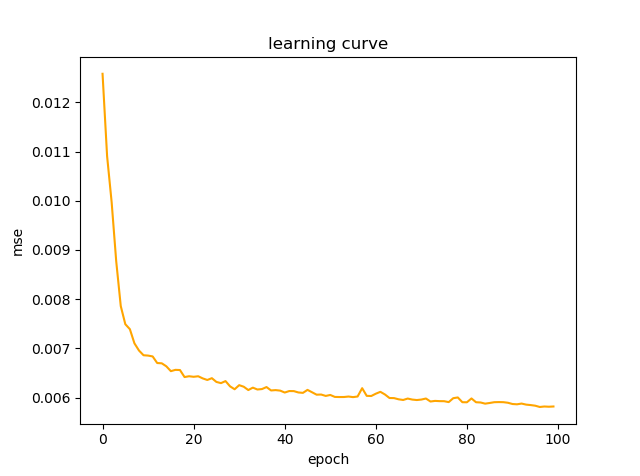
\includegraphics[width=\linewidth]{pics/mse_learncurve.png}
	\caption[Lernkurve des UNets zur fünf Minuten Vorhersage]{Die dargestellte Lernkurve bezieht sich auf die fünf Minütige Radarvorhersage mittels MSE. Zum Trainieren wurden 1900 Samples aus dem Jahr 2016 verwendet. Abgebildet ist der Validation-Loss welcher auf weitere 50 Samples berechnet wurde. Die ersten Epochen ist eine sehr starke Verbesserung des Fehlers zu erkennen, auch nach 100 Epochen scheint die Fehlerkurve noch zu fallen.}
	\label{mseLC}
\end{figure}

Die erste Analyse der Lernkurve \ref{mseLC} zeigt, dass das Netz den Fehler (MSE) während der ersten 20 Epochen sehr stark verbessern kann. Auch bei der letzten Epoche scheint der Validation-Loss noch weiter zu fallen. Für dieses Einstiegsbeispiel soll das Ergebnis aber zunächst genügen. Es gilt noch zu klären, ob das Netz auch tatsächlich eine sinnvolle Vorhersage liefert und ob es in der Lage ist die Baseline zu schlagen. 

\begin{figure}[h]
	\centering
	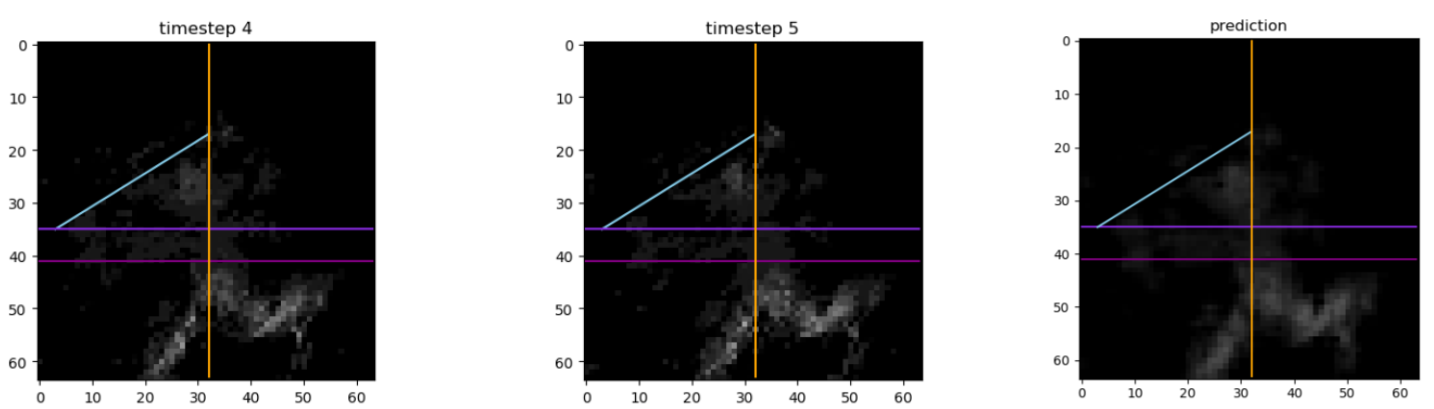
\includegraphics[width=\linewidth]{pics/mse_vgl1.png}
	\caption[Radarbilder für fünf-minuten Vorhersage]{Hier abgebildet sind mehrere Radarbilder. Je heller ein Pixel dargestellt ist, desto stärker regnet es an dieser Stelle. Das hier als timestep 4 bezeichnete Bild ist das letzte Eingangs-Bild und spiegelt somit die Baseline wieder. Rechts daneben abgebildet ist das Label, welches fünf Minuten später repräsentiert. Ganz rechts ist die Vorhersage des Netzes zu sehen. Die eingezeichneten Linien dienen nur der Orientierung um ein Vergleich der Bilder sowie das schätzen der Bewegung der Regenfront zu ermöglichen. Es ist deutlich zu sehen, dass Die Vorhersage des Netzes stark verschwommen ist. Die Bewegung der Regenwolken wurde allerdings sehr gut vorhergesagt. }
	\label{mse_VGL1}
\end{figure}

Die Ausgabe sowie die Baseline sind in Abbildung \ref{mse_VGL1} für ein Validierungssample zu sehen. Das Netz hat die Bewegung der Regenfront gut vorhergesagt, allerdings ist die Regenintensität meist unterschätzt. Vor allem starken Niederschlag kann das Netz nicht vorhersagen. Das ist in der linken Abbildung an den weißen Punkten unten Links gut zu erkennen. Das Netz sagt hier eher einen dunkleren Grauton als das Label vorher. Um dennoch bewerten zu können, ob das Netz im Schnitt besser als die Baseline ist, wird für beide Vorhersagen der mittlere quadratische Fehler zum Label (im Bild 'timestep 5') berechnet. Das Resultat zeigt für die Baseline einen Fehler von 0.00165 und für das Netz etwa 0.0008. Die Baseline macht im Schnitt also einen doppelt so großen Fehler wie unser Netz. Diese Berechnung wurde für alle 50 Validierungssamples vorgenommen. Das Resultat ist in Abbildung \ref{vglBaseline1} zu sehen.

\begin{figure}[h]
	\centering
	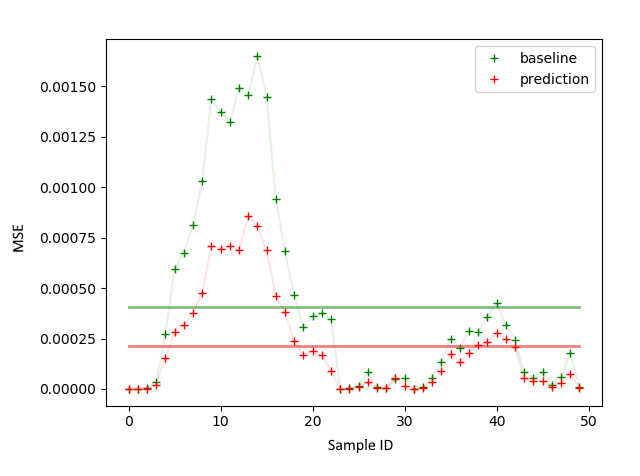
\includegraphics[width=\linewidth]{pics/mse_baseline.png}
	\caption[Vergleich zwischen Baseline und Netzvorhersage.]{Auf der X-Achse sind die 50 Validierungssamples aufgelistet. Die Y-Achse entspricht dem MSE. Für jedes Sample wurde der MSE jeweils für die Vorhersage des Netzes (rot) und der Vorhersage der Baseline (grün) berechnet. Die Performance der Baseline konnte überboten werden.}
	\label{vglBaseline1}
\end{figure}

Einige Validierungsdaten konnten nahezu ohne Fehler vorhergesagt werden. Dies sind Bilder, bei welchen kein Regen mehr in dem Label zu sehen ist. Hat auch die Baseline keinen Fehler gemacht, war bereits im letzten Zeitschritt kein Regen mehr vorhanden. Alle anderen Samples beinhalten Regenwetter in den Labels. Hier ist die Baseline auch durchgehend schlechter. Dies kommt vor allem daher, dass sich Regenfronten sowohl verschieben, als auch die Regenmenge innerhalb fünf Minuten deutlich wechseln kann. selbst eine Verschiebung von lediglich einem Pixel resultiert in einem deutlichen Fehler.

Als nächsten Schritt wollen wir die Performance des Netzes noch weiter Steigern. Hierzu werden verschiedene Ansätze versucht. Die zugehörigen Lernkurven sind in Abbildung \ref{lc_unet_types} zu sehen.
Die bisher verwendete Architektur ist in Blau eingezeichnet. Der erste Versuch war es das Output-Layer statt mit einem 1x1 Kernel mit einem 3x3 Kernel auszustatten um regionale Einflüsse besser in das Ergebnis mit aufzunehmen. Das Ergebnis hiervon ist ein vor allem Anfangs deutlich schnelleres sinken des Fehlers. Nach 80 Epochen ist die Performance nur geringfügig besser. Ein weiterer Versuch ist das erweitern des Netzwerkes um eine neue Ebene. Diese Ebene besteht wieder aus 20 3x3 Kernel, das nun tiefere Netzwerk ist in Grün dargestellt und erreicht die selbe Performance wie das ursprüngliche Netz. eine deutliche Vergrößerung der neuen Schicht (von 20 auf 60 Kernel) kann die Performance minimal verbessern. Die zugehörige Lernkurve ist in Rot eingezeichnet. Ein anderer Ansatz ist das ersetzen der ReLU Aktivierungsfunktionen durch Sigmoid Aktivierungsfunktionen. Hierdurch erhöht sich der Rechenaufwand enorm, da die ReLU lediglich negative Werte abschneidet und eine Sigmoid-Funktion für jeden Wert einen neuen Funktionswert berechnen muss. Die Performance ist in Violett eingezeichnet und zeigt keine Verbesserung. Auch die Fehlerfunktion wird testweise ausgetauscht, statt dem MSE wird der MAE verwendet, welcher lediglich ohne Quadrate arbeitet. Aber auch hier (Braune Kurve) ist keine Verbesserung zu erkennen. Als letztes wird der Adam-Optimizer ausgetauscht. Die Alternative ist der Nestreov-Optimizer, welcher in der Lernkurve (Pink) deutliche Sprünge aufweist. Eine nennenswerte Änderung konnte allerdings mit keiner Optimierung erreicht werden. lediglich ein Unterschied in der Rechenzeit ist bemerkbar. Da die Netze zeitweise auch auf der CPU trainiert werden müssen, Da benötgte Hard- und Software nur teilweise während des Projekts zur Verfügung standen, wird weiterhin das Blaue bisher verwendete UNet verwendet.

\begin{figure}[h]
	\centering
	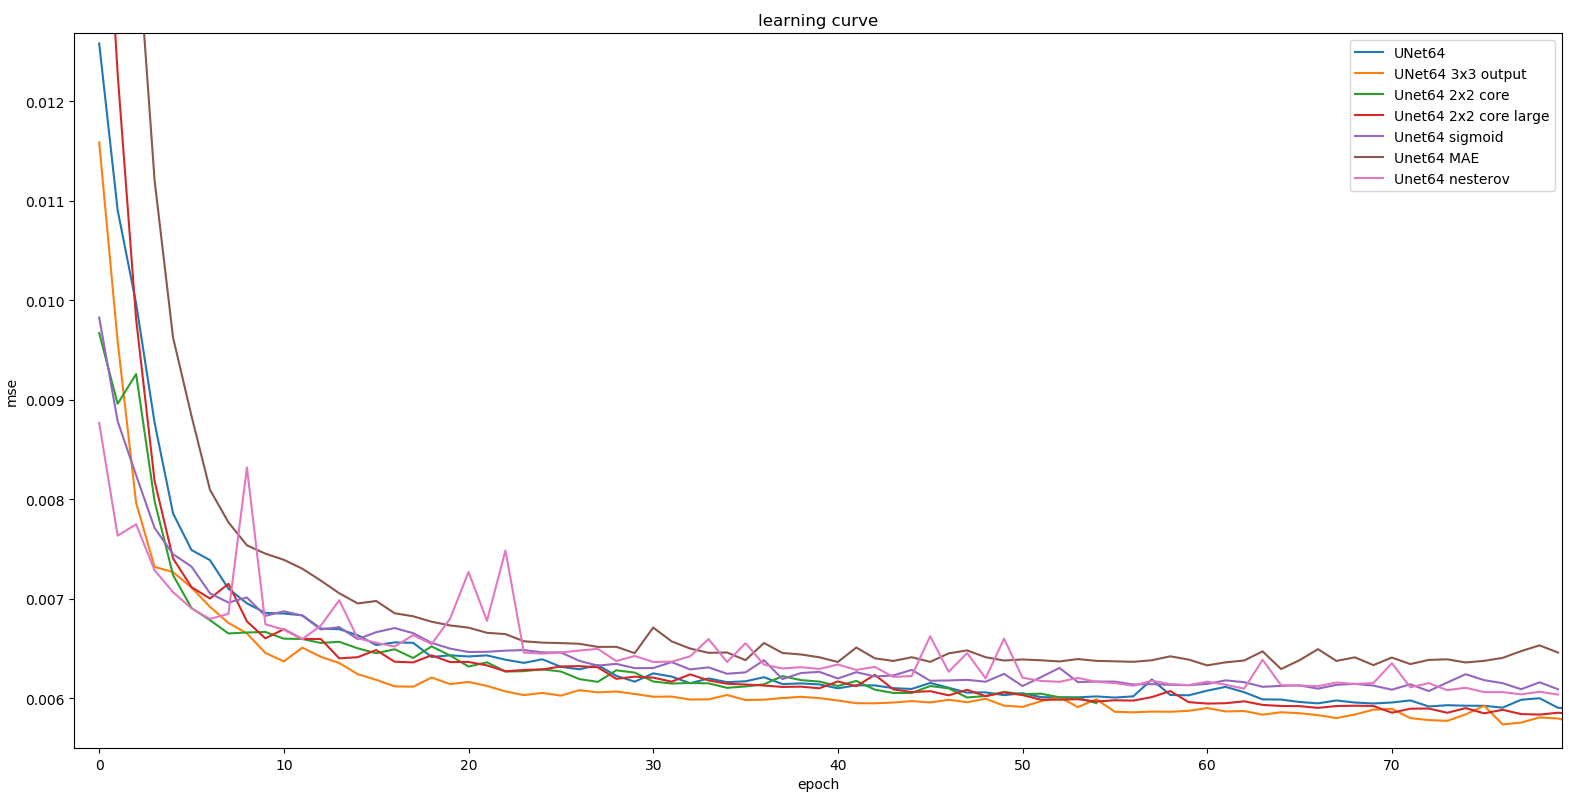
\includegraphics[width=\linewidth]{pics/vgl_lc_optim.png}
	\caption[Verschiedene UNet optimierungen im Vergleich.]{
		Um die Performance unserer UNet-Architektur weiter zu steigern wurden unterschiedliche Änderungen versucht. Die blaue Kurve zeigt das bisher verwendete Netz. Ein größerer Kernel am Output-Layer (gelb) verbessert die Performance ein wenig. Eine tiefere Netzwerkarchitektur (grün) steigert die Performance erst bei verwenden von sehr vielen Kernel (rot). Das Austauschen der Aktivierungsfunktionen gegen eine sigmoid-Funktion (violett) ändert außer an der Berechnungsgeschwindigkeit nichts. Das Austauschen der Fehlerfunktion gegen den MAE (braun) sowie das ändern des Optimierers zum Nesterov (pink) zeigen keine Verbesserung. Insgesamt werden nur deutliche Änderungen an der Rechenzeit festgestellt. Die Ergebnisse bleiben von der Performance vergleichbar.
		}
	\label{lc_unet_types}
\end{figure}

% -> Mehrere Zeitschritte vorhersagen
\subsection{Fünfunddreißig Minuten vorhersage}
Da die Baseline also mit dieser Architektur geschlagen werden kann, ist das nächste Ziel mehr als nur 5 Minuten vorherzusagen. Die hierfür verwendeten Daten bestehen aus 7 Zeitschritten im Label, also bis zu 35 Minuten in die Zukunft. Die Netzarchitektur muss hierfür lediglich am Output-Layer angepasst werden. Hierzu wird der 1x1 Kernel gegen sieben 1x1 Kernel ausgetauscht. Die Fehlerfunktion bleibt wie bisher der MSE, eine unterschiedliche Gewichtung der Zeitschritte wird nicht vorgenommen.
Für das Training wird nun auf alle zur Verfügung stehenden Daten zugegriffen. Dies entspricht 7500 Trainings- und 623 Validierungssamples.

\begin{figure}[h]
	\centering
	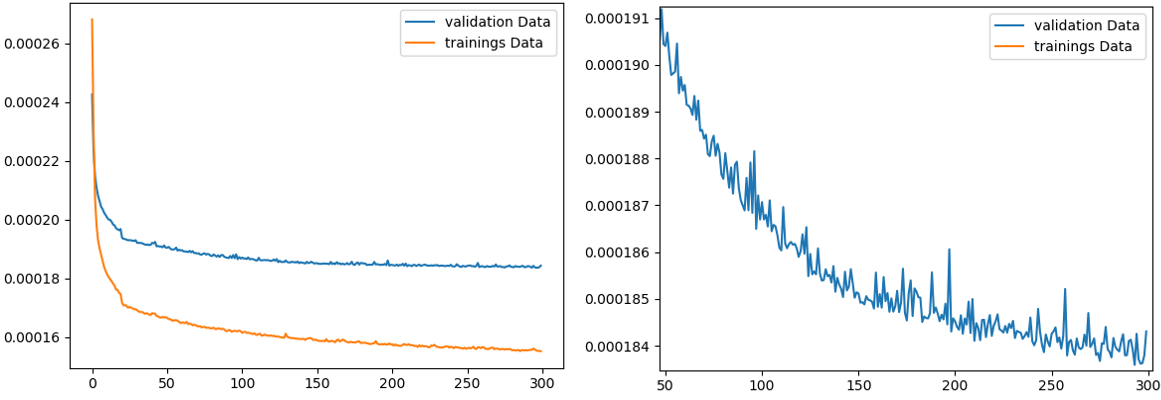
\includegraphics[width=\linewidth]{pics/lc_35minMSE.png}
	\caption[Lernkurve des UNet zur 35 Minuten Radar-Vorhersage.]{Die abgebildete Lernkurve zeigt, dass das Netz erst nach ca. 300 Epochen sich nicht weiter verbessert. Die rechte Abbildung ist ein Ausschnitt aus der linken, bei welcher das fallen der Lernkurve besser sichtbar ist.}
	\label{lc_35minMSE}
\end{figure}

Die zugehörige Lernkurve ist in Abbildung \ref{lc_35minMSE} zu sehen. Da die Performance auf das Validierungsset (blaue Kurve) nicht weiter verbessert wird, kann mit der Auswertung begonnen werden.
Zunächst wird das Netz wieder mit der Baseline verglichen. Hierfür wird jeder Zeitschritt aus dem Label mit dem letzten Zeitschritt der Eingabe-Daten verglichen. Da die Baseline davon ausgeht, dass das Wetter so bleibt wie es ist, ist zu erwarten, dass die Baseline mit zunehmender Zeit stets schlechter wird. Auch das Netz sollte mit zunehmender Zeit Probleme bekommen die Daten noch korrekt vorherzusagen. Eine direkter Vergleich pro Zeitschritt zwischen Baseline und Netzvorhersage wird in Abbildung \ref{35vglbasepred} dargestellt.
Die obere Zeile der Abbildung enthält die Verteilung der Vorhersage, während die untere Zeile die der Baseline enthält. Die Spalten geben die Zeitschritte an, zwei untereinander liegende Histogramme stellen die selbe Zeitliche Vorhersage dar. 
In den Histogrammen ist die Verteilung der Summe der quadratischen Fehler für alle Validierungsdaten dargestellt. Es wurde also pro Vorhersage eine Summe über alle quadratischen Abweichungen zwischen Vorhersage und Label, pro Zeitschritt, berechnet.
Schwarz eingezeichnet ist der Mittelwert, die beiden grauen Linien entsprechen dem 25\%-, bzw 75\%-Quantil. Es ist deutlich zu erkennen, dass der Mittelwert des Fehlers mit zunehmender Zeit größer wird, bzw. nach rechts wandert. Dies war so auch zu erwarten, da mit zunehmender Zeit stets neue Faktoren Einfluss auf das Wetterverhalten haben. Interessanter ist der Vergleich der Spalten. Der Mittelwert des Fehlers ist durchgehend besser bei der Vorhersage des Netzes als bei der Baseline. Mit zunehmender Zeit wird dieser Unterschied allerdings sehr gering.

\begin{figure}[h]
	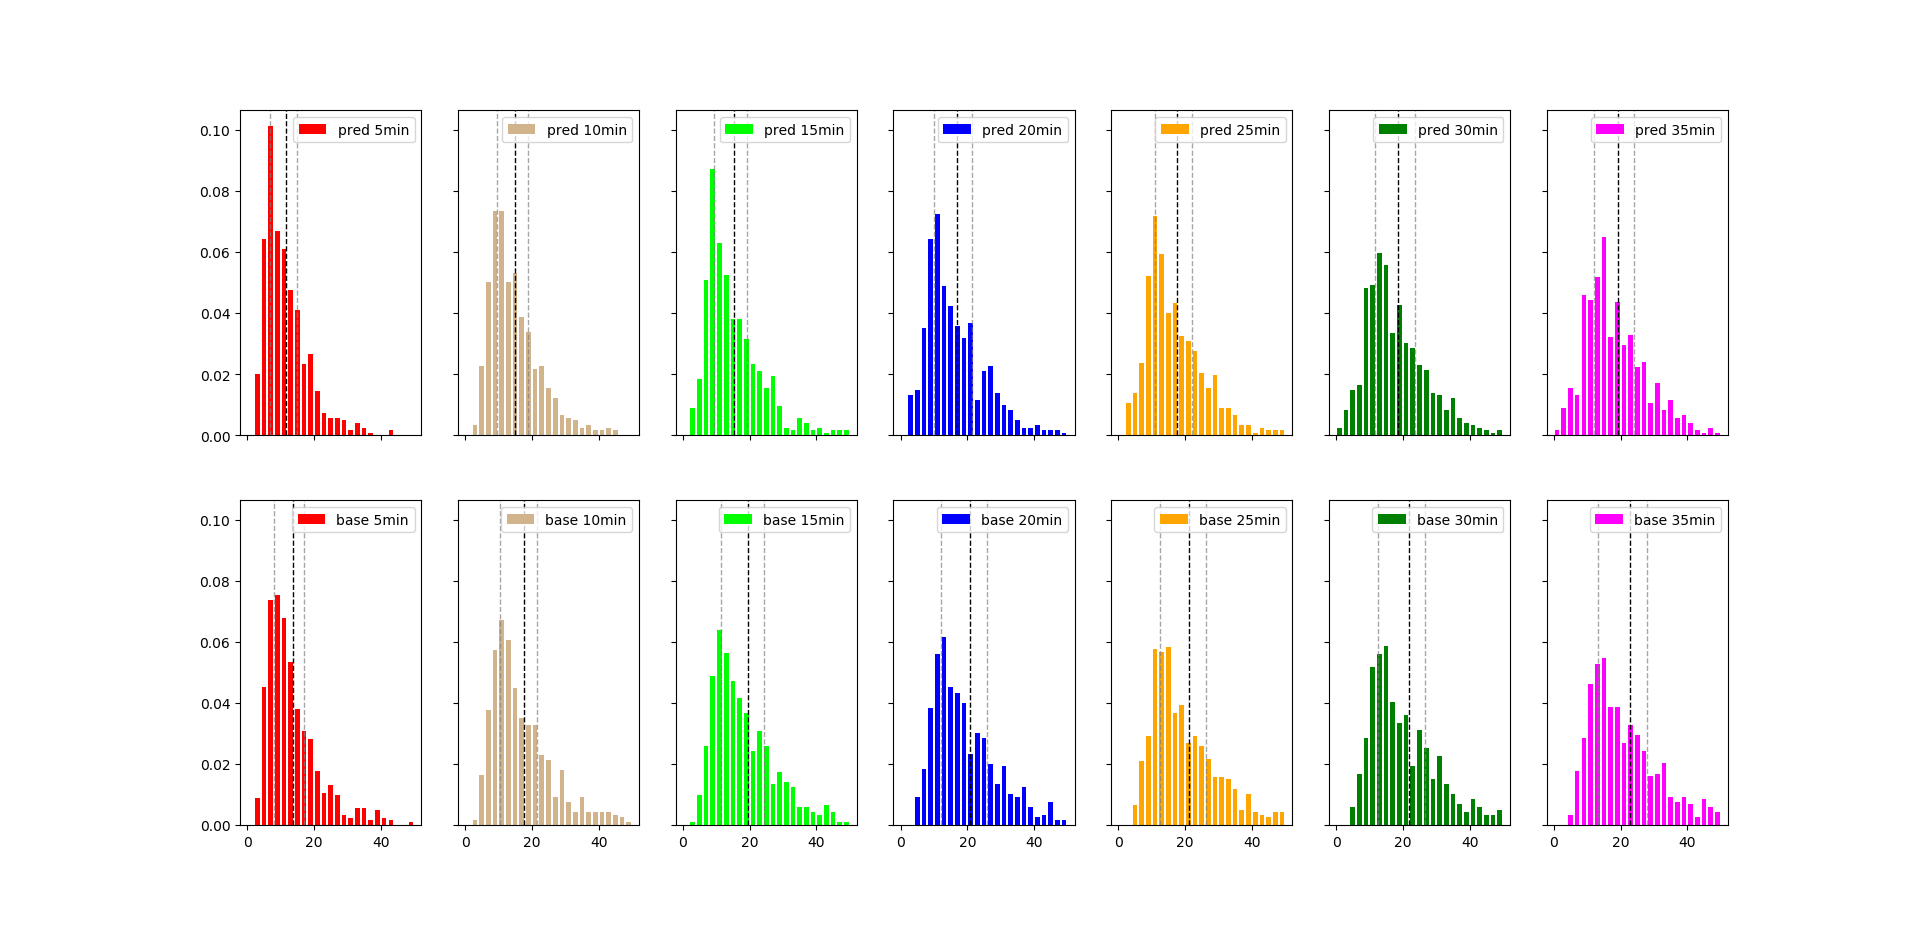
\includegraphics[width=\linewidth]{pics/35min_vgl_baseline.png}
	\caption[Vergleich zwischen Baseline und UNet (35 Minuten Vorhersage)]{Ein Vergleich zwischen Baseline und Vorhersage. In den Spalten sind die Zeitlichen Schritte von 5 bis 35 Minuten Vorhersage. In der oberen Zeile ist die Vorhersage des Netzes und in der unteren die der Baseline abgebildet. Die Histogramme zeigen die Summe der Quadratischen Fehler pro Zeitschritt. Die schwarzen Linien zeigen den Mittelwert der Verteilung, während die grauen Linien das 25\%- sowie das 75\% Quantil darstellen. Mit zunehmender Zeit wandert die Verteilung weiter nach rechts, die Vorhersagen stimmen also weniger mit dem Label überein.}
	\label{35vglbasepred}
\end{figure}

Den Zahlen nach ist das Ziel die Baseline zu schlagen also geschafft. Um aber wirklich ein Fazit ziehen zu können werden die Daten und Vorhersagen in nachfolgender Abbildung \ref{vieleBilder1} und \ref{vieleBilder2} dargestellt.
Die hier verwendeten Daten und Label entstammen dem Validierungsset, welches Radardaten aus dem Jahr 2014 umfasst. sie wurden in keinem Trainingsschritt verwendet.
Die Abbildungen zeigen deutlich, dass das Netz die ersten fünf Minuten sehr genau vorhersagen kann. Das ausgegebene Bild hat unterschiedliche Niederschlagsmengen für jeden Pixel vorhergesagt. Mit zunehmender Zeit lässt diese Genauigkeit aber stark nach. So ist im letzten Ausgabebild sehr häufig für einen ganzen Bereich die selbe Niederschlagsmenge vorhergesagt. Es wirkt, als würde die Auflösung der Vorhersage mit zunehmender Zeit abnehmen. Durch die schwache Auflösung werden viele Pixel nicht ganz korrekt wiedergegeben, was den Fehler erhöht. Der so entstehende Fehler ist aber dennoch geringer, als der Fehler welchen die Baseline macht, indem sie exakte Niederschlagsmengen für jeden Pixel vorhersagt. Unser Netz schlägt die Baseline also nicht dadurch eine exaktere Vorhersage zu treffen, sondern durch eine verschwommene Regenfront, welche sich entsprechend der eingegangenen Daten weiter bewegt und dabei auch stets auseinander driftet.


\begin{figure}[ht]
	\centering
	\begin{subfigure}[]{\linewidth} 
		\centering
		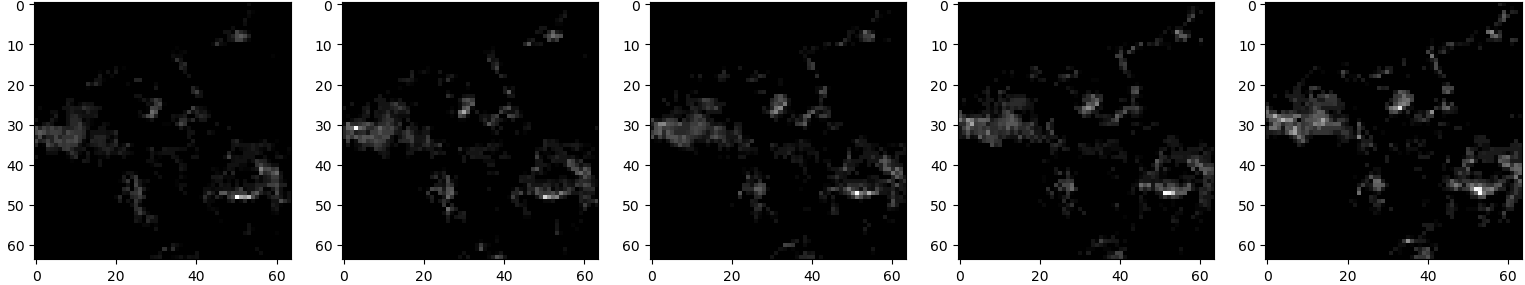
\includegraphics[width=\linewidth]{pics/dt2.png}
		\caption[]{}\label{fa}
	\end{subfigure}
	
	\begin{subfigure}[]{\linewidth} 
		\centering
		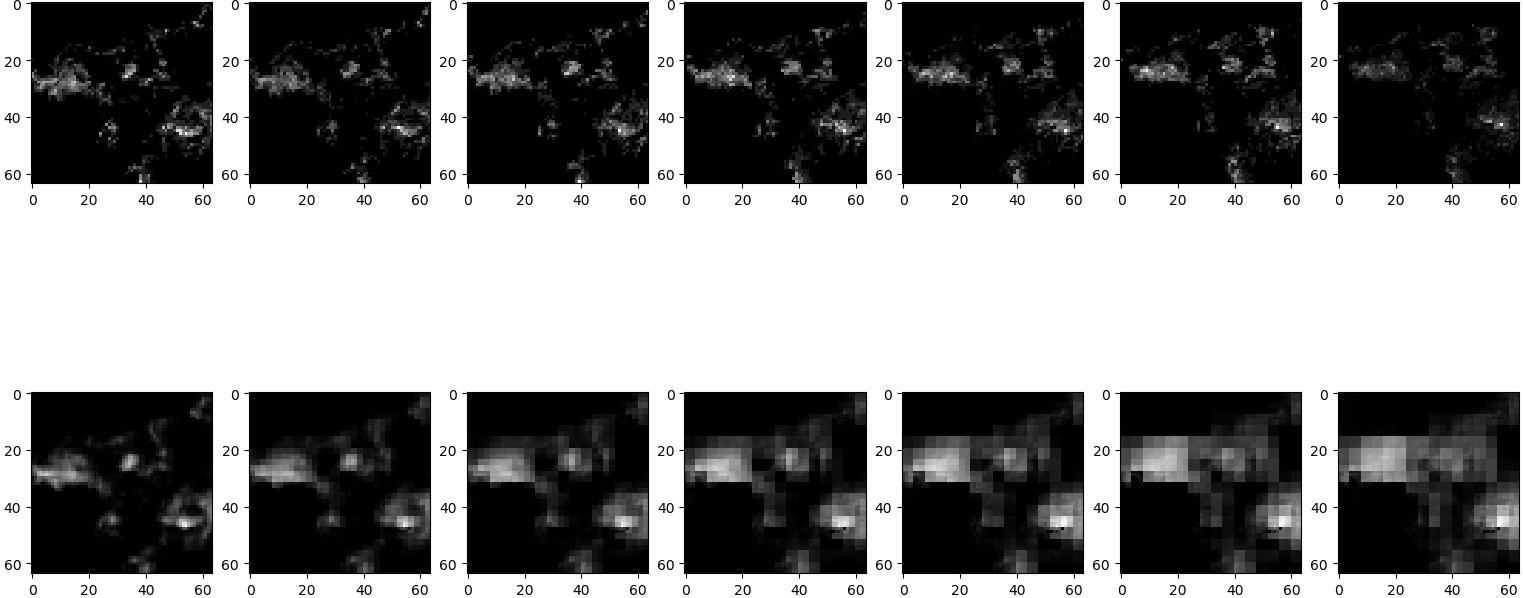
\includegraphics[width=\linewidth]{pics/t2.png}
		\caption[]{}\label{fb}
	\end{subfigure}
	
	\caption[Validierungsdaten und Label sowie Vorhersage 1]{Die in (a) gezeigten Bilder entsprechen den eingehenden 25 Minuten an Radardaten. In (b) sind die 35 Minuten Label sowie darunter die 35 Minuten Vorhersagen abgebildet. Mit zunehmender Zeit wird die Vorhersage ungenauer. Während das erste Bild das Label noch gut wiedergeben kann, besteht das siebte nur noch aus sehr groben Strukturen.}
	\label{vieleBilder1}
\end{figure}

\begin{figure}[ht]
	\centering
	\begin{subfigure}[]{\linewidth} 
		\centering
		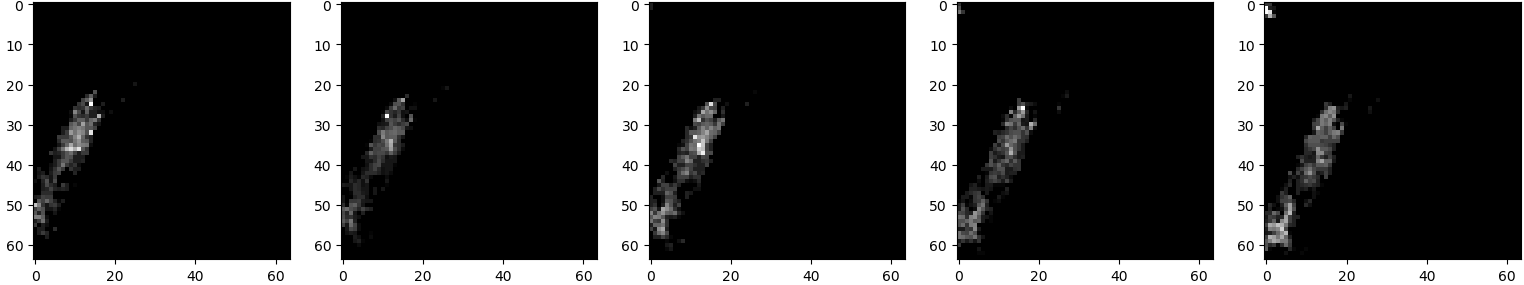
\includegraphics[width=\linewidth]{pics/dt5.png}
		\caption[]{}\label{ga}
	\end{subfigure}
	
	\begin{subfigure}[]{\linewidth} 
		\centering
		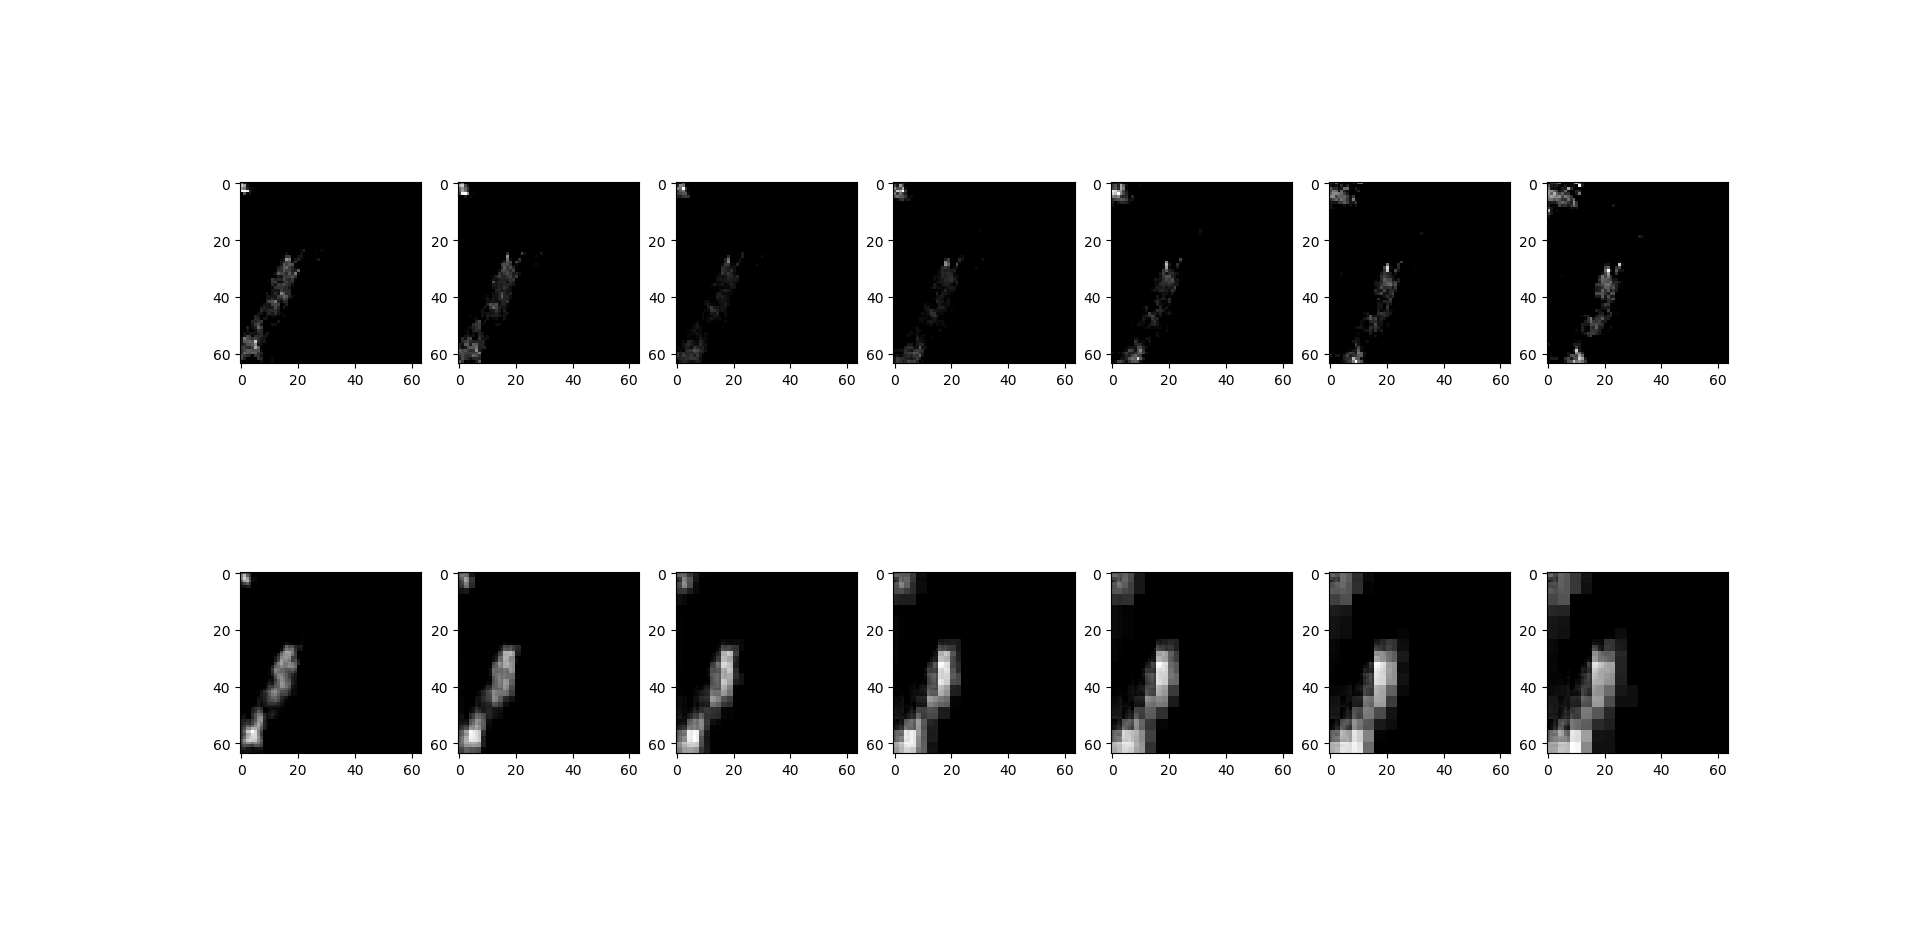
\includegraphics[width=\linewidth]{pics/t5.png}
		\caption[]{}\label{gb}
	\end{subfigure}
	
	\caption[Validierungsdaten und Label sowie Vorhersage 2]{Die in (a) gezeigten Bilder entsprechen den eingehenden 25 Minuten an Radardaten. In (b) sind die 35 Minuten Label sowie darunter die 35 Minuten Vorhersagen abgebildet. Im Gegensatz zu Abbildung \ref{vieleBilder1} kann hier anhand der oberen linken Ecke sehr gut eine Bewegung wahrgenommen werden. Obwohl die Regenfront erst in den letzten beiden Eingabebildern erscheint, kann sie in den sieben Ausgabebildern vorhergesagt werden. Zwar ist auch hier die Vorhersage sehr ungenau, aber die Bewegungsrichtung ist korrekt vorhergesagt.}
	\label{vieleBilder2}
\end{figure}


%wie gut zum nicht nass werden ?
% zum ende Kommen...
%ToDo: vgl mit Zeros?
%ToDo: Daten/Label erzeugung einfuegen -> \label{Samples}
%ToDo: Auch 5Daten1Label bild einbinden -> \label{5D1L}

